\clearpage
\section{Compound  Nouns Analysis} \label{nominals}
The second example of a language construct that causes problems for machine reading in the absence of background knowledge 
arises from the use of compound nouns. Noun phrases contain a number of challenging compositional
phenomena, including implicit relations.
  Compound nouns such as ``pro-choice Democratic gubernatorial candidate
James Florio'', or ``White House spokesman Marlin Fitzwater'' primarily consist of  nouns and adjectives. They do not contain verbs. 
This means that it is difficult for a pattern detection algorithm to detect any useful lexical regularities across compound nouns that express the same relations.   On the other hand, beliefs such as a person’s job title, nationality, or stance on a political issue
are often expressed using compound nouns. We  propose a knowledge-aware algorithm for extracting semantic relations from compound noun analysis that learns, through distant supervision, to  map fine-grained type sequences of compound nouns to the relations they express.
Consider the following compound nouns. 



\begin{table}[h]
%
\centering
%
\begin{tabular}{ll}
\hline
1.a) Giants	cornerback	Aaron Ross \\
1.b) Patriots	quarterback	 Matt Cassel \\
1.c) Colts	receiver	Bryan Fletcher \\
\hline
2.a)  Japanese	astronaut	Soichi Noguchi \\
2.b) Irish	golfer	Padraig Harrington \\
2.c) French	philosopher	Jean-Paul Sartre \\
\hline
2.a) Seabiscuit	author	Laura Hillenbrand \\
2.b) Harry porter author J.K Rowling \\
2.c) Walking the Bible author Bruce Feile \\
\end{tabular}
%\caption{Example of nominals }
%\tom{What does "-" mean in this table?  If zero, let's use "0"}}
\label{tab:nominalsexamples}
\end{table}
     

The concepts in the  compound noun sequences \textit{(1a. -- c.)}, \textit{(2a. -- c.)}, \textit{(3a. -- c.)}  are
of the semantic type sequences:

\begin{table}[h]
%
\centering
%
 \begin{tabular}{ll}
   \hline
\textit{\textless sportsteam\textgreater \textless sportsteamposition\textgreater \textless athlete\textgreater}  \\
\textit{\textless country\textgreater \textless profession\textgreater \textless person\textgreater} \\
\textit{\textless book\textgreater  ``author" \textless person\textgreater} \\
        \hline
 \end{tabular}
 %\caption{Example of nominals }
 %\tom{What does "-" mean in this table?  If zero, let's use "0"}}
   \label{tab:nominalstypesequences}
 \end{table}
     
     

Therefore, our task is to learn semantic type sequences and their mappings to knowledge base relations. In our case we use relations from the NELL knowledge base. Since  NELL has   binary relations that  take only two arguments, and compound nouns contain more than two noun phrases,  we additionally keep track of the position information for the two arguments of the relation.  For example, from the type sequence:   \textit{\textless country \textgreater \textless profession\textgreater \textless person\textgreater}, we generate mappings to two different  relations.

\begin{table}[h]
\begin{tabular}{llll}
\hline
\textbf{Relation}&  \textbf{arg1\_pos} &  \textbf{arg2\_pos} & \textbf{type sequence} \\
\hline
citizenofcountry & 3 & 1 & \textit{\textless country\textgreater \textless profession\textgreater \textless person\textgreater} \\
personhasjobposition & 3 & 2 & \textit{\textless country\textgreater \textless profession\textgreater \textless person\textgreater} \\
     \hline
\end{tabular}
\caption{Learned mappings from compound nouns semantic type sequences to binary relations }
%\tom{What does "-" mean in this table?  If zero, let's use "0"}}
\label{tab:nominalsmappings}
\end{table}

\begin{figure}[t]
%
\centering
%
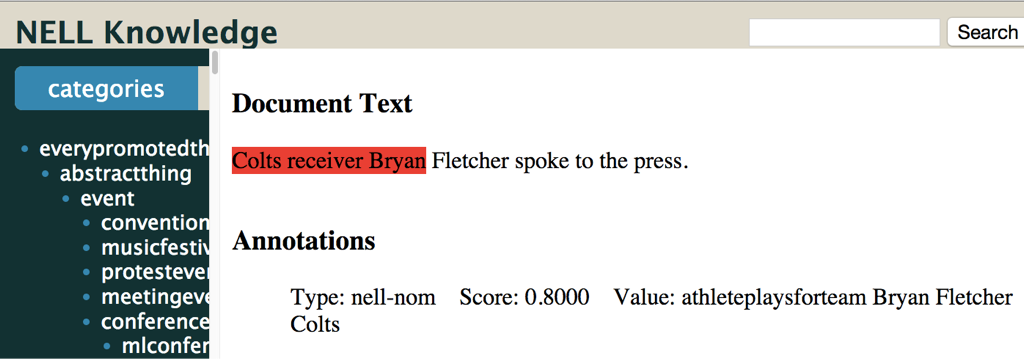
\includegraphics[width=1\columnwidth] {athletenominal.png}
%
%\vspace*{-1cm}
\caption{Extracting the athleteplaysforteam relation from a compound noun.}
%
\label{fig:athletenominal}
%
\end{figure}

To learn  mappings from  compound nouns to binary relations as shown in Table \ref{tab:nominalsmappings}, we  use  distant supervision, that is using the NELL knowledge base as the only form of supervision.   In general, the intuition behind
 distant supervision is that a sentence that contains a pair of entities that participate in a known
knowledge relation is likely to express that relation. In our case, the sentence is just a compound noun. Therefore, we first extract compound nouns from a large collection of documents.  For every compound noun,  we map its noun phrase to entities in the NELL. The entities are then replaced by their NELL types. This creates  type sequences of the form:  \textit{\textless country \textgreater \textless profession\textgreater \textless person\textgreater}.  Each type sequence has a support set, which is the collection of  compound nouns that satisfy the type sequence. For example, a support compound noun might be: \textit{Japanese	astronaut	Soichi Noguchi}   for the type sequence: \textit{\textless country\textgreater \textless profession\textgreater \textless person\textgreater}.  We retain type sequences whose support set sizes are above a threshold of  $10$ in our experiments.  For  type sequences with support set size above the threshold, we use their support sets to learn mappings from type sequences to relations using distant supervision.  That is, from each supporting compound noun we collect pairs of entities, and do look ups in NELL to determine which relations hold between the pair of entities. We additionally keep track of the position of  the entities within the compound noun. This gives us mappings from types sequences to relations such as:  \textit{\textless citizenofcountry\textgreater \textless3\textgreater  \textless1\textgreater \textless country\textgreater \textless profession\textgreater}. We only retain mappings that have a support set size (relation instances in NELL) above a threshold of $10$ in our experiments.

\subsection{Experimental Evaluation}
We extracted compound nouns from three different corpora: the New York
Times archive which includes about 1.8 Million
 articles from the years 1987 to 2007, the English edition of Wikipedia  with about
about 3.8 Million articles, and the KBP dataset \cite{conf/tac/Surdeanu13} which contains over 2 million documents with  Gigaword newswire  and Wb documents. We extracted a total of $2,270,487$ compound nouns.
From these compound nouns, we  extract 10 relations that are expressed by compound nouns and are in the NELL knowledge base. From this dataset we learned 291 mappings from  types sequences to relations.  Using these mappings we then predicted new relation instances. We report  recall and accuracy   in  Table \ref{tab:nominalsresult}. We can see that this approach has high accuracy across all the relations. Recall is also high for certain relations but low for others. This might be because  certain relations although they are expressed using compound nouns, they are more commonly expressed in other forms.

We have incorporated this system into the NELL reading software. A screenshot of extracting relations from compound nouns is shown in Figure \ref{fig:athletenominal}.



\begin{table}[h]
%
\centering
%
 \begin{tabular}{l|l|l}
 \hline
 Relation & Recall & Precision \\
   \hline
   citizenofcountry & 15,805 &$0.982\pm0.018$ \\
citylocatedincountry & 1,521 & $0.75\pm0.083$ \\
athleteplaysforteam &471 & $0.982\pm0.018$ \\
persongraduatedfromuniversity& 49 & $0.964\pm0.036$ \\
personhasjobposition & 511,937 & $0.837\pm0.07$ \\
musicianplaysinstrument & 3,890 & $0.885\pm0.06$ \\
worksfor & 75,757 &  $0.847\pm0.068$ \\
athletewinsawardtrophytournament & 92 & $0.928\pm0.049$ \\
coachesteam& 175 & $0.982\pm0.018$ \\
companysubsidiary& 37 & $0.953\pm0.047$ \\
   \hline
 \end{tabular}
 \caption{Recall and  precision of relation extraction for 10 relations. Precision is sampled
 from a total of max(100, recall).}
 %\tom{What does "-" mean in this table?  If zero, let's use "0"}}
   \label{tab:nominalsresult}
 \end{table}





    
\subsection{Related Work}
Much of the work on information extraction has been on extracting relations expressed by verb phrases
that occur between pairs of noun phrases. Extracting knowledge base relations from noun phrases alone has been much less
explored. In \cite{conf/emnlp/YahyaWGH14}, a method is  developed that learns noun phrase
structure for open information extraction. This is different from our work in that we are extract 
knowledge base relations as opposed to open information extraction. Therefore, the authors
do not ground their extracted attributes to an
external knowledge base. 


The work of \cite{choi2015scalable} developed a semantic parser for extracting relations
 from noun phrases. Given an input noun phrases, it is first transformed to a logical form, where the logical form is an 
 intermediate unambiguous representation of the noun phrase.
The  logical form is chosen such that it  closely matches the linguistic structure
of the input text noun phrase. The logical form is then transformed into one that, where possible,
uses the Freebase ontology predicates \cite{Bollacker2008}. These predicates can then be read off as relations expressed about the 
entities described by the noun phrase. The authors test their work on Wikipedia category names. Since each Wikipedia category
describes a set of entities, by extracting relations from each category name, one learns relations about all the members of the category.
Consider the Wikipedia category \textit{Symphonic Poems by Jean Sibelius}.  An example of the knowledge base transformed  logical form for this category name would be: 

$\lambda x.composition.form(x;Symphonic$ $poems) \wedge composer(Jean$ $Sibelius; x)$ where one can now extract attributes for the entities, such as \textit{The Bard, Finlandia, Pohjola’s Daughter, En Saga, Spring Song, Tapiola, \ldots},  that 
fall under this category  in particular that for all $x$ in this category $composer(Jean$ $Sibelius; x)$ and  $composition.form(x; Symphonic$ $poems)$
where $composer$ and $composition.form$ are Freebase attributes. In generating the logical forms, several features are used that capture some background knowledge, in particular,   a number of features that enable soft
 type checking on the  produced logical form, and  features that test agreement of these
 types on different parts of the produced  logical form.
 
In a related but different line of work,  the NomBank project  \cite{conf/lrec/MeyersRMSZYG04,conf/acl/GerberC10} annotated the argument
structures for common nouns. For example, from the expression \textit{Greenspan’s replacement Ben Bernanke},
the arguments for the nominal ``replacement", are: ``Ben
Bernanke" is  ARG0 and ``Greenspan" is  ARG1. The resulting annotations
has been used as training data for work on semantic role labeling on nominals \cite{jiang2006semantic,conf/acl/LiuN07}.
Again, this work is different from our work in that no knowledge base relations are extracted.


There has  also  work on the broader topic of semantic structure of noun phrases. In \cite{conf/acl/SawaiSM15}, a method is proposed that parsers noun phrases into the Abstract Meaning Representation in order to detect the argument structures, and noun-noun relations in compound nouns.


\subsection{Compound  Noun Analysis Summary}
We have presented a knowledge-aware method for relation extraction from 
compound nouns.   Our method uses semantic types of concepts in compound noun sequences
to predict relations expressed by novel compound noun sequences containing concepts that we have not seen before. This  method can be
seen as another example of tapping into a positive feedback loop for machine reading made possible by projects that construct large-scale knowledge bases. Compound nouns are non-trivial to interpret in many different ways besides the noun-noun relations problem we addressed here.  For example, one problem that could benefit from background knowledge is that of   analyzing the internal structure of noun phrases through bracketing \cite{conf/acl/VadasC07,conf/acl/VadasC08}.  For example, in the noun phrase \textit{(lung cancer) deaths},  the task would be to determine that  \textit{lung cancer} modifies the head \textit{deaths}. Additionally, as future work we can increase our predicate vocabulary to learn more common sense type of relations from compound nouns, for example, in the noun phrase \textit{cooking pot}, we can extract the relation\text{purpose}, to mean the pot is used for cooking.
 


